\chapter{Autonomous Driving as a Representative Application}
\label{sec:application}
% ============================================


% Springer Nature: each chapter should have a 10--15 line online abstract.
% This chapter abstract has not yet been written in the uploaded manuscript.
\abstract*{}
\suppressfloats[t]

Autonomous driving is a representative high-complexity application of sensor fusion because it brings together heterogeneous sensing, real-time operation, uncertainty management, safety-critical decision-making, and strict deployment constraints. It is not the only domain in which sensor fusion is required, but it provides a particularly useful case study because many general fusion challenges appear simultaneously within a complete cyber--physical system. In this section, autonomous driving is therefore used to illustrate how the theoretical principles and algorithmic methods discussed in the previous sections are instantiated in practice.

\section{System Context and Sensor Suite}

An autonomous vehicle must estimate both its external environment and its own state. To do so, it combines exteroceptive sensors, which observe the surrounding scene; proprioceptive sensors, which measure ego-motion; and external or cooperative information sources, which provide global, map-based, or communication-assisted context. A representative sensor arrangement is shown in Fig.~\ref{fig:autonomous-vehicle-sensors-layout}.

\begin{figure}[!t]
    \centering
    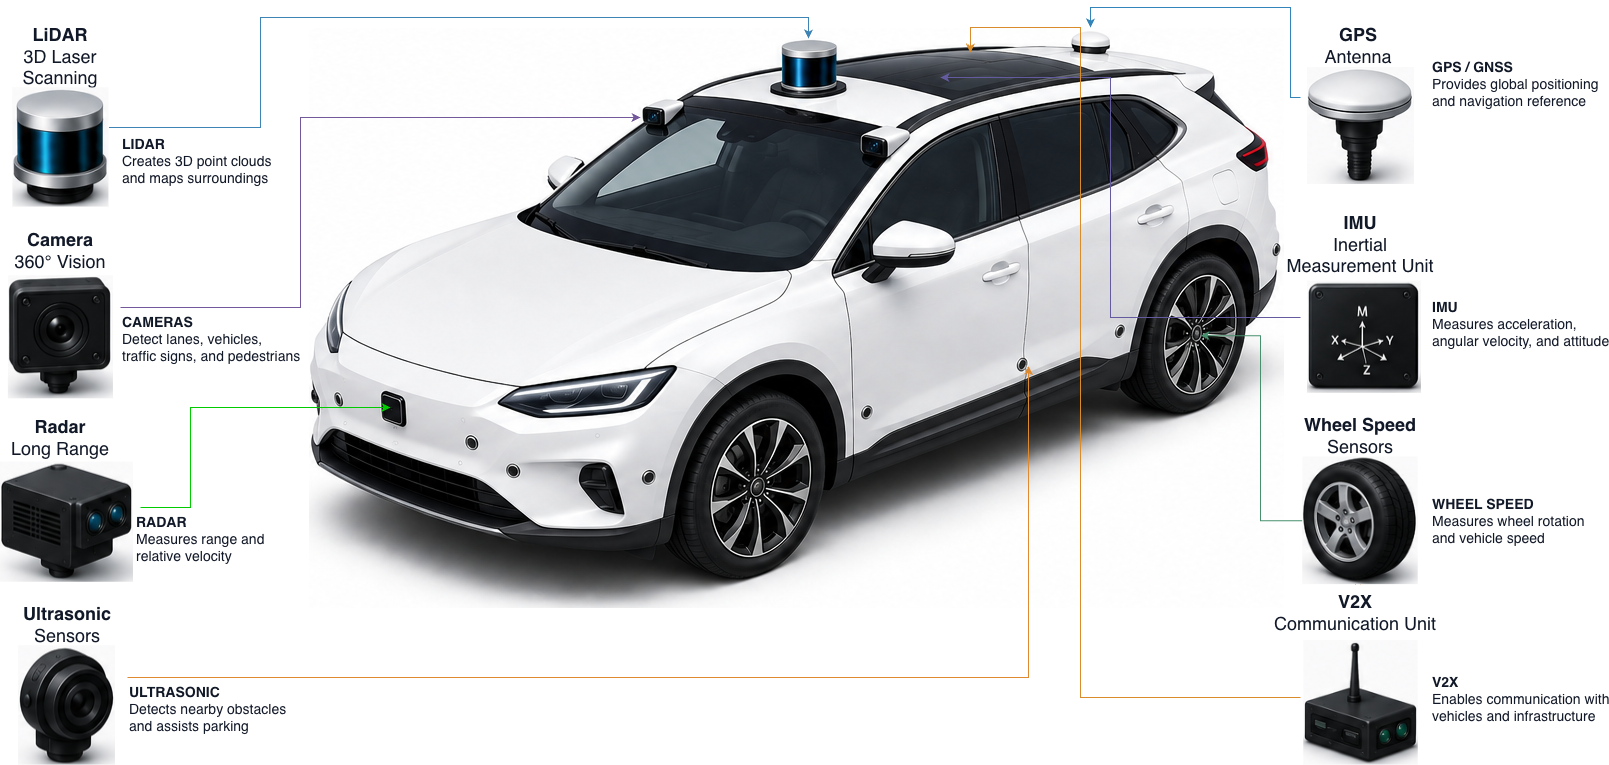
\includegraphics[width=\textwidth]{figures/autonomous_vehicle_sensors_layout_v02.png}
    \caption{Representative autonomous-vehicle sensor layout, showing complementary sensing modalities for perception, localisation, ego-motion estimation, short-range obstacle detection, and communication.}
    \label{fig:autonomous-vehicle-sensors-layout}
\end{figure}

The sensor layout in Fig.~\ref{fig:autonomous-vehicle-sensors-layout} highlights the complementarity that motivates autonomous-driving sensor fusion. The strengths, limitations, and typical fusion roles of the individual modalities are summarised in Tables~\ref{tab:av-onboard-sensors} and~\ref{tab:av-cooperative-inputs}; here we only note the overall pattern: cameras contribute semantics, LiDAR contributes geometry, radar contributes range and velocity under poor visibility, ultrasonic sensors cover the near field, IMUs and wheel odometry provide high-rate ego-motion subject to drift, and GNSS, maps, V2X, and roadside infrastructure extend awareness beyond the onboard field of view.

These modalities are not interchangeable. Instead, each provides a different type of information, with different uncertainty, sampling rate, field of view, latency, and failure modes. Autonomous-driving fusion therefore aims to exploit both \emph{complementarity}, where one sensor provides information that another cannot, and \emph{redundancy}, where multiple sensors observe related aspects of the same scene and can be used for consistency checking, robustness, and fault tolerance.

Table~\ref{tab:av-onboard-sensors} summarises common onboard sensing modalities, while Table~\ref{tab:av-cooperative-inputs} summarises cooperative, localisation, and map-based inputs that support autonomous-driving fusion.

\begin{table}[!t]
    \centering
    \small
    \caption{Onboard sensing modalities commonly used in autonomous-driving sensor fusion.}
    \label{tab:av-onboard-sensors}
    \begin{tabular}{p{0.08\linewidth} p{0.28\linewidth} p{0.30\linewidth} p{0.25\linewidth}}
        \hline
        \textbf{Sensor} & \textbf{Strengths} & \textbf{Limitations} & \textbf{Typical Fusion Role} \\
        \hline
        Camera & Dense appearance, colour, texture, lane markings, traffic signs, traffic lights, and semantic cues & Sensitive to lighting, glare, shadows, night-time conditions, adverse weather, and limited direct depth estimation & Semantic perception, object classification, lane detection, traffic-light recognition, image--LiDAR and image--radar fusion \\
        \hline
        LiDAR & Accurate 3D geometry, depth, object shape, road structure, and point-cloud representation & Higher cost, sparse at long range, affected by rain, fog, snow, and reflective surfaces & 3D object detection, mapping, localisation, free-space estimation, camera--LiDAR fusion \\
        \hline
        Radar & Long range, direct relative velocity, robustness to poor visibility and adverse weather & Lower angular resolution, multipath effects, ghost detections, noisier spatial structure & Object tracking, velocity estimation, long-range detection, radar--camera and radar--LiDAR fusion \\
        \hline
        Ultrasonic & Low-cost short-range sensing, useful for parking and close obstacle detection & Very limited range, low spatial resolution, affected by surface geometry and environmental noise & Low-speed manoeuvring, parking assistance, near-field obstacle detection \\
        \hline
        IMU & High-rate acceleration and angular velocity, useful for short-term ego-motion estimation & Biases and integration drift accumulate over time & Ego-motion prediction, inertial navigation, GNSS--IMU, visual--inertial, and LiDAR--inertial fusion \\
        \hline
        Wheel odometry & Direct vehicle motion information, low cost, high update rate & Accumulates drift, affected by wheel slip, tyre deformation, and road surface conditions & Dead reckoning, vehicle state estimation, GNSS--IMU--odometry fusion \\
        \hline
    \end{tabular}
\end{table}

\begin{table}[!t]
    \centering
    \small
    \caption{Cooperative sensing, localisation, and map-based inputs used in autonomous-driving fusion.}
    \label{tab:av-cooperative-inputs}
    \begin{tabular}{p{0.13\linewidth} p{0.26\linewidth} p{0.28\linewidth} p{0.24\linewidth}}
        \hline
        \textbf{Input} & \textbf{Strengths} & \textbf{Limitations} & \textbf{Typical Fusion Role} \\
        \hline
        GNSS & Provides global positioning in open-sky environments and supports absolute localisation & Degraded by tunnels, urban canyons, multipath, signal blockage, interference, and spoofing risks & Global localisation, correction of accumulated drift in GNSS--IMU, GNSS--wheel odometry, and map-based localisation \\
        \hline
        High-definition maps & Provide prior information about lanes, road boundaries, intersections, landmarks, traffic rules, and road topology & Can become outdated, require accurate localisation, and are costly to build, update, and maintain & Map matching, lane-level localisation, perception priors, planning context, road-structure reasoning \\
        \hline
        V2X communication & Extends perception beyond line of sight and can provide information from nearby vehicles, infrastructure, and traffic-management systems & Depends on connectivity, latency, standardisation, trust, cyber-security, and communication coverage & Cooperative perception, hazard warning, traffic-signal information, occlusion handling, extended situational awareness \\
        \hline
        Roadside infrastructure sensors & Provide external viewpoints from fixed cameras, LiDARs, radars, or smart-city infrastructure & Require deployment and maintenance, depend on communication links, and raise calibration, synchronisation, privacy, and security issues & Infrastructure-assisted perception, validation, cooperative tracking, scenario recording, ground-truth-like reference generation \\
        \hline
    \end{tabular}
\end{table}

\section{Fusion Pipeline and Architectural Levels}

Sensor fusion appears at several points in the autonomous-driving pipeline. A typical system includes sensing, calibration and synchronisation, preprocessing, perception, localisation and mapping, tracking, prediction, planning, and control. Measurements from cameras, LiDAR, radar, ultrasonic sensors, IMUs, wheel encoders, GNSS receivers, maps, V2X messages, and infrastructure sensors must first be temporally synchronised and spatially aligned. This usually requires intrinsic calibration, extrinsic calibration, timestamp correction, latency compensation, motion compensation, and coordinate-frame transformations.

Figure~\ref{fig:autonomous-driving-fusion-pipeline} illustrates the main stages of a typical autonomous-driving sensor-fusion pipeline. The important point is that fusion is not confined to a single block. It can occur repeatedly at different abstraction levels and for different purposes.

\begin{figure}[!t]
    \centering
    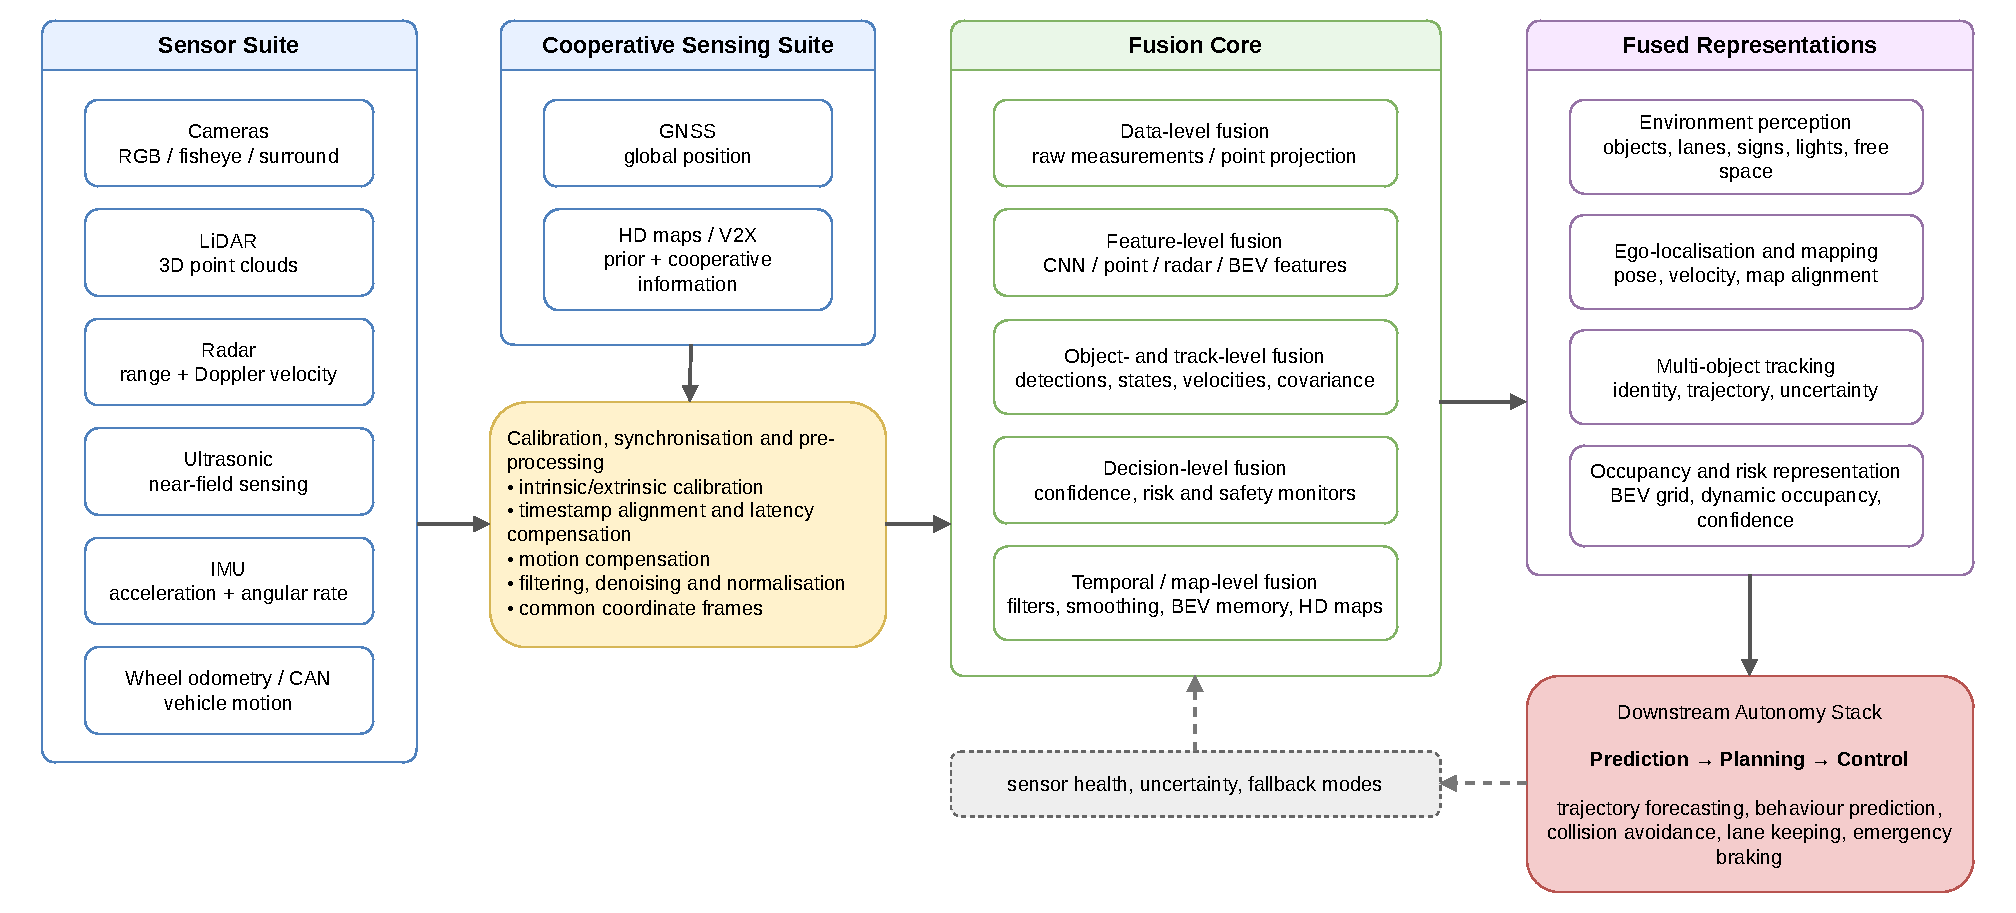
\includegraphics[width=\textwidth]{figures/autonomous_driving_fusion_pipeline.pdf}
    \caption{Autonomous-driving sensor fusion pipeline. Heterogeneous sensor measurements are calibrated, synchronised, and pre-processed before being fused at data, feature, object, decision, temporal, and map levels. The fused representations support environment perception, ego-localisation, mapping, tracking, occupancy estimation, prediction, planning, and control.}
    \label{fig:autonomous-driving-fusion-pipeline}
\end{figure}

Data-level fusion combines low-level measurements directly, for example by projecting LiDAR points into the image plane, aggregating multiple LiDAR sweeps, or associating radar detections with point-cloud clusters. Feature-level fusion combines extracted or learned representations, as in camera--LiDAR, camera--radar, LiDAR--radar, and bird's-eye-view neural architectures. Object- and track-level fusion combines detections, bounding boxes, velocities, class probabilities, covariances, and track states across sensors. Decision-level fusion combines classifier outputs, risk scores, occupancy decisions, or safety-monitoring signals. Temporal fusion uses filtering, smoothing, recurrent networks, temporal attention, or memory-based BEV representations to integrate information over time. Map-level fusion aligns online sensor observations with high-definition maps or previously built local maps.

This layered view clarifies why autonomous driving is a demanding fusion problem. The vehicle must combine onboard exteroceptive sensing for environment perception, proprioceptive sensing for ego-motion estimation, global and map-based references for localisation, and cooperative information for extended situational awareness \cite{2023:IEEE_ITSM,TANG2023109165}. These inputs must then be transformed into representations that are useful for downstream prediction, planning, and control. Errors in calibration, synchronisation, data association, uncertainty modelling, or sensor reliability estimation can therefore propagate through the entire autonomy stack.

\section{Core Fusion Tasks}

Autonomous-driving fusion supports several core tasks. The first is environment perception, where cameras, LiDAR, radar, and maps are used to estimate drivable space, lanes, road boundaries, traffic signs, traffic lights, vehicles, cyclists, pedestrians, and other obstacles. LiDAR depth can improve the spatial accuracy of image-based segmentation, while image semantics can improve the interpretation of sparse point clouds. Radar can contribute long-range range-rate information, especially for moving objects and adverse-weather scenarios. Map priors can further help distinguish valid road areas, pavements, junctions, and lane-level structure.

A second major task is three-dimensional object detection and tracking. Camera--LiDAR fusion is widely used for accurate 3D bounding-box estimation and classification, while radar is valuable for long-range detection and velocity estimation. Tracking extends detection over time by maintaining object identity, position, velocity, acceleration, heading, and uncertainty. Classical filters, smoothing methods, data-association algorithms, and track-management logic remain important even when the detections themselves are produced by deep neural networks.

A third task is ego-localisation and mapping. GNSS, IMU, wheel odometry, cameras, LiDAR, and high-definition maps are fused to estimate the vehicle's position and orientation relative to a local map, global frame, or lane-level map. GNSS alone is insufficient in tunnels, dense urban areas, and multipath environments, while inertial and odometry estimates drift over time. Visual, LiDAR, and map-based localisation can correct this drift, but must handle outdated maps, temporary roadworks, changed lane layouts, perceptual aliasing, and localisation uncertainty.

A fourth task is occupancy, free-space, and risk estimation. Instead of representing the scene only as a list of detected objects, occupancy-based fusion estimates which regions of space are free, occupied, unknown, or dynamically occupied. Risk-aware fusion can incorporate object uncertainty, time-to-collision, occlusion regions, road boundaries, predicted future occupancy, and traffic-rule constraints. These representations are especially important for prediction and planning because the planner must act not only on what is detected, but also on what may be hidden, uncertain, or about to enter the vehicle's path.

Robustness is central to all of these tasks. Rain, fog, snow, darkness, glare, dust, road spray, sensor contamination, and unusual traffic behaviour affect modalities differently. Reliability-aware fusion can adjust sensor weights according to environmental conditions and sensor-health indicators, while temporal fusion can reduce transient false positives and improve consistency. However, fusion cannot compensate for all failures. If several modalities degrade simultaneously, or if the scene lies outside the training or design distribution, the fusion system must detect its own uncertainty and support conservative fallback behaviour.

\section{Datasets, Metrics, and Evaluation}

Public datasets have played a major role in autonomous-driving fusion research. Common benchmarks include KITTI, nuScenes, Waymo Open Dataset, Argoverse, Lyft Level 5, ApolloScape, Oxford RobotCar, Cityscapes, A2D2, ONCE, and BDD100K\addednew{~\cite{geiger2013_kitti,caesar2020_nuscenes,sun2020_waymo,chang2019_argoverse,cordts2016_cityscapes,yu2020_bdd100k}}. These datasets differ in sensor suite, geographic coverage, weather diversity, annotation type, object classes, and supported tasks. A method developed on a camera--LiDAR dataset may not transfer directly to radar fusion, adverse-weather perception, infrastructure-assisted sensing, or map-based localisation. \addednew{Because the datasets named above are dominated by clear-weather scenes, adverse-condition and robustness-oriented benchmarks are increasingly necessary complements: the Seeing Through Fog dataset provides camera--LiDAR--radar recordings in fog, rain, and snow \cite{bijelic2020_stf}, while corruption suites in the style of RoboBEV systematically perturb inputs to probe how BEV fusion architectures degrade \cite{dong2023_robobev}. For a survey whose central claim is robustness through fusion, such benchmarks matter more than average-case leaderboards.} % [July 2026 pass] Dataset name-dropping without citations was a reviewer-visible gap; added citations and an adverse-weather benchmark note. Bib entries in references_additions.bib.

Fusion systems can be evaluated across 2D object detection, 3D object detection, semantic segmentation, panoptic segmentation, lane detection, free-space estimation, multi-object tracking, ego-localisation, odometry, mapping, occupancy prediction, and trajectory prediction. Detection tasks commonly use average precision and mean average precision, while segmentation tasks use intersection-over-union and mean intersection-over-union. Localisation and odometry are often evaluated using absolute trajectory error, relative pose error, drift, heading error, and map-matching accuracy. Tracking metrics additionally assess identity switches, track fragmentation, missed detections, false positives, and trajectory consistency.

For autonomous driving, average benchmark accuracy is not sufficient. Evaluation should also consider latency, throughput, memory footprint, energy consumption, hardware utilisation, uncertainty calibration, false-negative rates for vulnerable road users, robustness under degraded sensing, and performance in rare safety-critical scenarios. Scenario-based testing, simulation, hardware-in-the-loop evaluation, closed-course testing, and real-world trials are important complements to public benchmarks because many critical failures are rare, context-dependent, and difficult to capture in static datasets.

\section{Implementation and Validation}

A practical autonomous-driving fusion system requires more than the fusion algorithm itself. It also requires sensor drivers, calibration tools, data logging, synchronisation mechanisms, coordinate-frame management, visualisation tools, middleware, and deployment-aware software design. ROS and ROS2 are widely used for prototyping because they provide modular communication between sensor, perception, localisation, planning, and control nodes. Python is often used for rapid algorithm development and evaluation, while C++ is commonly used for performance-critical deployment. Deep learning frameworks such as PyTorch and TensorFlow are used for training and evaluating learning-based fusion models.

Practical systems must maintain consistent coordinate frames and timestamps throughout the processing pipeline. This typically requires calibration files, transform trees, time-offset estimation, motion compensation, and careful handling of missing, delayed, or out-of-order messages. Deployment platforms may include CPUs, GPUs, FPGAs, and heterogeneous embedded computing architectures. FPGA-based Kalman and LQG implementations illustrate how estimation cores can be accelerated and validated using hardware-in-the-loop frameworks \cite{deliparaschos_fpgabased_2016}. Such implementations are relevant because latency, energy consumption, and timing determinism become critical when fusion outputs directly affect planning and control.

Several implementation patterns illustrate the connection between fusion theory and deployment. GNSS--IMU--wheel odometry fusion uses inertial and odometry measurements for prediction and GNSS or map-based updates for drift correction. Camera--LiDAR feature-level fusion combines semantic image features with geometric point-cloud or BEV features for 3D perception. Radar--camera--LiDAR track-level fusion associates detections across modalities and maintains object states over time. Reliability-aware fusion adapts sensor weights according to visibility, blockage, timestamp delay, calibration quality, detection confidence, environmental condition, and sensor-health indicators.

System-level validation is essential because real-world fusion performance depends not only on the algorithm, but also on timing, sensor configuration, calibration quality, communication latency, compute resources, and interaction with downstream planning and control. Integrated testing and simulation infrastructures can evaluate sensor fusion components together with perception, control, and human-interaction models \cite{deliparaschos_preliminary_2020}. A concrete example is the Multi-User Environment for Autonomous Vehicle Innovation (MUEAVI), an integrated validation infrastructure for autonomous vehicles and smart-city transport. The facility combines physical road infrastructure, heterogeneous sensor networks, embedded edge processing, a central data-fusion centre, visualisation tools, scenario recording, and software-based validation \cite{deliparaschos_preliminary_2020}.

The MUEAVI camera-tracking pipeline illustrates how infrastructure-level sensing can be connected to perception and actuation through middleware. In this scenario, a full-HD video stream from a PTZ camera is decoded using the NVIDIA DeepStream framework, object detection and tracking are performed, object-detection messages are broadcast through Apache Kafka, and the \texttt{kafka\_ROS\_connector} node converts these messages into custom ROS messages. The \texttt{deepstream\_ptz\_control} node then computes relative pan--tilt--zoom commands from the detected-object list, while the \texttt{ptz\_control} node sends these commands to the PTZ camera and publishes camera status information \cite{deliparaschos_preliminary_2020}. Figure~\ref{fig:mueavi-camera-tracking} illustrates this camera-tracking control-loop validation scenario.

\begin{figure}[!t]
    \centering
    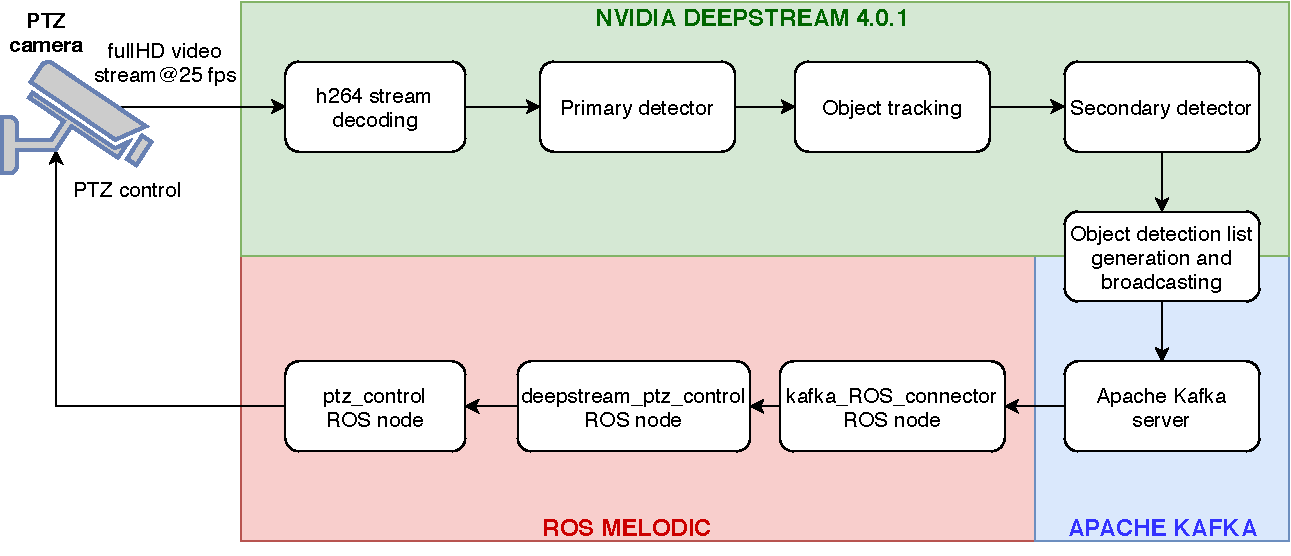
\includegraphics[width=\textwidth]{figures/tracking_with_camera.pdf}
    \caption{Camera tracking control-loop validation scenario based on the MUEAVI infrastructure. The pipeline receives a full-HD video stream from a PTZ camera, decodes it using the NVIDIA DeepStream framework, performs object detection and tracking, broadcasts object-detection messages through Apache Kafka, and converts these messages into ROS messages using the \texttt{kafka\_ROS\_connector} node. The \texttt{deepstream\_ptz\_control} ROS node computes relative pan--tilt--zoom commands from the detected-object list, while the \texttt{ptz\_control} ROS node sends the commands to the PTZ camera and publishes camera status information.}
    \label{fig:mueavi-camera-tracking}
\end{figure}

Infrastructure-supported fusion systems extend this idea by combining data from vehicle-mounted and fixed sensing sources. Roadside cameras, LiDARs, and radars can observe vehicles and vulnerable road users from viewpoints that differ from those available to the ego vehicle. This can improve object tracking, support cooperative perception, provide external validation for onboard perception, and help analyse occluded or safety-critical scenarios.

A representative infrastructure-assisted architecture consists of three layers. The first layer performs local acquisition and preprocessing close to the sensors, including video decoding, timestamping, point-cloud filtering, radar parsing, clustering, and object detection. Camera-based detection can be implemented using real-time neural detectors such as YOLOv3 \cite{redmon_yolov3_2018}. LiDAR and radar preprocessing commonly involves point-cloud filtering, downsampling, segmentation, and clustering, with tools such as the Point Cloud Library and algorithms such as DBSCAN being widely used in practical implementations \cite{rusu_pcl_2011, ester_dbscan_1996}. The second layer performs centralised or distributed fusion, including coordinate transformation, multi-object tracking, object classification, sensor-selection logic, and scenario classification. The third layer supports validation, visualisation, data storage, and comparison against simulation or reference measurements.

This type of architecture connects sensor fusion with verification and validation rather than treating it as an isolated perception module. It also exposes practical implementation issues that are often hidden in algorithm-only descriptions, including time synchronisation, multi-sensor cross-calibration, middleware design, network latency, edge-computing constraints, and real-time data storage. Hardware--software co-design and systematic sensor-selection methods are therefore relevant when fusion algorithms must be deployed on embedded or resource-constrained platforms \cite{deliparaschos_fpga_2016}.

% ============================================
